\documentclass[12pt]{article}
\usepackage[a4paper, margin=2cm]{geometry}
\usepackage[english]{babel} % To obtain English text with the blindtext package
\usepackage{blindtext}
\usepackage{graphicx} % Required for inserting images
\usepackage{array, multirow} % For extra column formatting
\usepackage{amsmath, amssymb, cancel} %for equation environment
\usepackage{float}
\usepackage{parskip} % For gaps between para
\usepackage{setspace}
\usepackage{pdfpages}
\usepackage{abstract}
\usepackage{longtable}
\usepackage[export]{adjustbox}
\usepackage{emptypage}
\usepackage{tocloft}
\usepackage[nottoc]{tocbibind}
\usepackage{hyperref, url}
\usepackage[table]{xcolor}
\usepackage{minted}
    \usemintedstyle{monokai}
\usepackage{caption}
    \captionsetup{font=footnotesize,labelfont=bf}
\usepackage{tcolorbox}
    \newtcolorbox{mintedbox}{
        colback=backcolour,
        boxrule=0pt,
        sharp corners,
        width=\linewidth,
        left=0pt, right=0pt,
        top=3pt, bottom=3pt
    }

\cftsetindents{section}{0em}{2em}
\cftsetindents{subsection}{0em}{2em}

\renewcommand\cfttoctitlefont{\hfill\Large\bfseries}
\renewcommand\cftaftertoctitle{\hfill\mbox{}}

\graphicspath{ {./images/} }

\pagenumbering{arabic}

\definecolor{blurple}{HTML}{5865F2}
\definecolor{backcolour}{HTML}{272823}

\hypersetup{
    colorlinks=true,
    linkcolor=black,
    urlcolor=blurple,
    citecolor=blurple,
}

\urlstyle{same}

\renewcommand{\arraystretch}{1.4}

\setcounter{secnumdepth}{5}
\setcounter{tocdepth}{5}
\newcommand\simpleparagraph[1]{%
  \stepcounter{paragraph}\paragraph*{\theparagraph\quad{}#1}}

%%%%%%%%%%%%%%%%%%%%%%%%%%%%%%%%%%%


\title{PHYC20040 Exp.2 Pleiades SM}
\author{Joana Adao}
\date{\today}

\begin{document}

\begin{titlepage}
    \begin{center}

        \begin{figure}[ht]
            
\includegraphics[width=\textwidth]{UCDLogo.png}
        \end{figure}
        
        \begin{figure}
            \centerline{
\includegraphics[width=\paperwidth]{UCDBanner.png}}
        \end{figure}

        \vspace{4cm}

        {\LARGE \bfseries PHYC20040 Exploring the Solar System}\\
        \vspace{0.75cm}
        {\Large Experiment No.3 The Classification of Stellar Spectra}
        
        \vspace{1cm}
    
    {\Large \textbf{26 February 2025}}

    \vspace{2cm}
    
    {\large \textbf{by Joana C.C. Adao (Student No. 23311051)}}\\

    \end{center}
    
   \clearpage

\end{titlepage}

\setcounter{page}{1}
\tableofcontents

\newpage

\begin{abstract}
\addcontentsline{toc}{section}{Abstract}

This experiment made use of the CLEA (Contemporary Laboratory Experience in Astronomy) \textit{'Classifying Stellar Spectra'} software to practice classifying a star's spectral type.
The program had a list of 25 pre-determined stars that were analysed and classified on their spectral type based off of their absorption spectra when compared to the known
spectra of main sequence stars from O-type to M-type. When these estimated spectral types were cross-checked to the spectral types as defined by the SIMBAD database and JHC Atlas,
\textbf{30.4\%} and \textbf{45.8\%} of the results matched, respectively. The same process was done for randomly selected stars in the simulated nightsky offered by CLEA, and these chosen
stars were compared to ones available on the SIMBAD database via input of their coordinates. 

\end{abstract}

%%%%%%%%%%%%%%%%%%%%%%%%%%%%%%%%%%%

\vspace{2.5cm}

\section{Theory} \label{sec:1}

\subsection{Spectra}

The electromagnetic spectrum describes all forms of electromagnetic radiation, including visible light, as it varies with wavelength
and frequency  
\cite{britspectra,hubblespectra}.
Spectroscopes are equipments used to visually observe the spectra and spectrographs photograph and map the studied spectra
\cite{britspectra}.
There are three main ways that the spectra can be classified, as illustrated in figure \ref{fig:spectra} \cite{spectrapic}.

\begin{figure}[H]
    \centering
    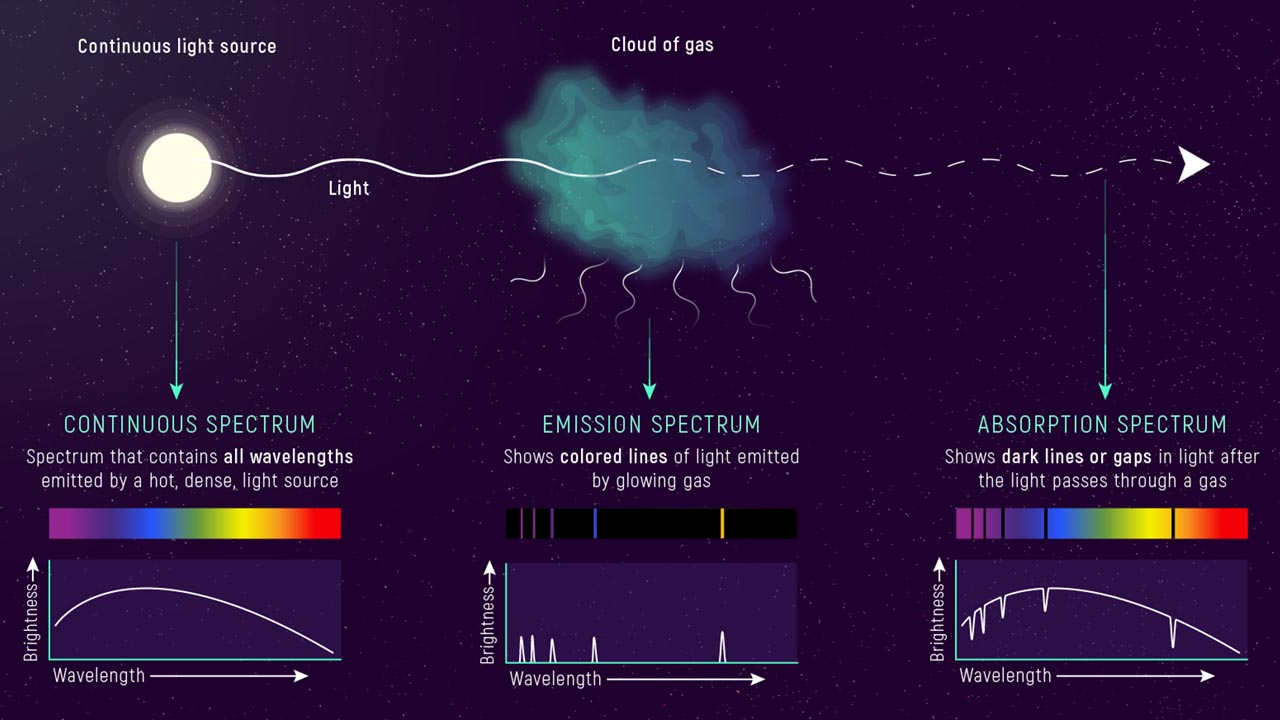
\includegraphics[width=15cm]{spectra.jpg}
    \caption{\centering \footnotesize{Types of spectra: continuous, emission, absorption \protect\cite{spectrapic}}}
    \label{fig:spectra}
\end{figure}

\textbf{Spectrometry} puts quantitative values to the theory explored by spectroscopy (\textit{theoretical} interaction between radiation and matter) by measuring the interactions between light (electromagnetic radiation)
and matter
\cite{ataspectrosco}.

\subsubsection{Absorption Line Spectra}

\textbf{The absorption spectrum} is measured when light from a continuous source, like a star, passes through a cloud of cooler gas.
The wavelengths that will be absorbed depend on the composition and elements of the gas, as well as its temperature and density. The wavelengths
that didn't pass through are what appear as dark lines on the continuous spectrum known as the absorption line spectrum \cite{cosmosabsorp}.

\subsubsection{Emission Line Spectra}

\textbf{The emmission spectrum} is measured when atoms become excited after light, like from a star, passes through a cloud of gas.
The light can heat up the cloud of gas, thus exciting the atoms and causing them to release light. The light which the gas releases depends on the
composition and elements, temperature, and density of the gas cloud. The light emitted will appear as coloured lines.

\subsection{Blackbody Radiation} \label{sec:1.1}

Blackbodies are idealised surfaces that can absorb any wavelenght of incident radiation without any reflection, and that can emit electromagnetic (EM) radiation
at maximum possible monochomatic intensities for a range of wavelengths (a continuous spectrum) based on temperature
\cite{librablackodyrad,UCDblackbocdyrad,ESAblackbodyrad}.

\begin{figure}[H]
    \centering
    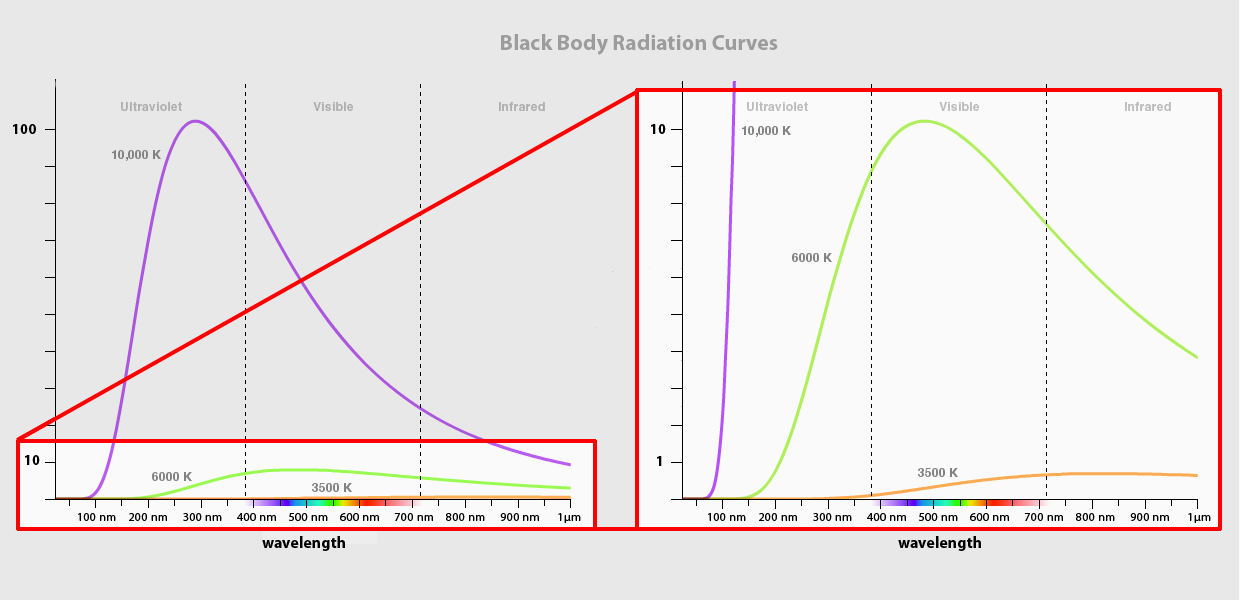
\includegraphics[width=12.5cm]{blackbody.jpg}
    \caption{\centering Diagram of blackbody radiation curves for stars of 10 000K, 6 000K, 3 500K, with the visible light spectrum shown on the x-axis \protect\cite{ESAblackbodyrad}.}
    \label{fig:blackbodyrad}
\end{figure}

The characteristic curve of the continuous spectrum of blackbody radiation can be used to determine the temperatures of stars and other cosmic objects by finding their "colour" \cite{ESAblackbodyrad}.
Hotter stars emit shorter wavelengths and therefore appear bluer, while colder stars emit longer wavelengths and therefore appear redder (see figure \ref{fig:msgraphspec}).


\subsubsection{Wien's Displacement Law}

Wien's Law relates the peak wavelength of a blackbody's peak emission spectrum ($\mathbf{\lambda_{peak}}$) to temperature (\textbf{T}) \cite{derivwien}.
This is given by the following, with $\mathbf{\lambda_{peak}}$ in metres (m) and temperature \textbf{T} in Kelvin (K) \cite{derivwien}:

\vspace{-1.5ex}
\begin{gather}
    \lambda_{peak} (\text{m}) = \frac{2.89777 \times 10 ^{-3}}{T} 
\end{gather}

The wavelength $\mathbf{\lambda_{peak}}$ can also be found in Ångstroms (Å) by changing the numerator constant to be in Ångstrom-Kelvin instead of metre-Kelvin:

\vspace{-1.5ex}
\begin{gather}
    \lambda_{peak} (\text{\AA}) = \frac{2.9 \times 10^7}{T}
\end{gather}

\vspace{1.5cm}
\subsection{Apparent and Absolute Magnitude} \label{sec:1.1.3}

Magnitude is a logarithmic measure of the brightness of a star or other celestial body. The brighter the object, the lower the magnitude (number), and they can be negative for particularly bright stars
\cite{britmag}.
The magnitude of the celestial objects are divided into two types of observation:

\begin{itemize}
    \item \textbf{Apparent magnitude, m,} is used to describe how bright a celestial object appears from the view on Earth
    \cite{lcomag}.
    \item \textbf{Absolute magnitude, M,} also in reference to \textbf{\textit{luminosity}}, is defined as the magnitude of the star if the distance between it and Earth were 10 parsecs (pc)
    \cite{lcoabsmag,cosmosabsmag}.
    When at a set distance, astronomers are then able to compare intrinsic brightness of stars
    \cite{cosmosabsmag}.
\end{itemize}

Absolute (\textbf{M}) and apparent (\textbf{m}) magnitudes can be used in equation \ref{eq:1} to calculate \textbf{D}, the distance in parsecs (pc).
The distance modulus is then $\mathbf{m - M}$.  The magnitudes do not have units
\cite{cosmosabsmag}.

\vspace{-1.5ex}
\begin{gather} \label{eq:1}
    M = m + 5 - 5 (\log_{10} D) \quad , \quad m - M = 5 \log_{10} \left( \frac{D}{10} \right)
\end{gather}

The above equation (\ref{eq:1}) can then be manipulated to find the distance, \textbf{D}:

\vspace{-1.5ex}
\begin{gather} \label{eq:2}
    \log_{10}D = \frac{m - M + 5}{5} \quad \implies \quad D = 10^{\frac{m - M + 5}{5}}
\end{gather}

\vspace{1.5cm}
\subsection{Stellar Classification}

\subsubsection{Harvard Classification of Spectral Types} \label{sec:1.2.1}

The currently-used system of classification of stars was created by a team at Harvard in 1924 \cite{harvardstar}. The different classes are \textbf{OBAFGKM}, left to right: hottest to coolest.
The different classes and temperature thresholds are illustrated in figure \ref{fig:starclassy}.

\begin{figure}[H]
    \centering
    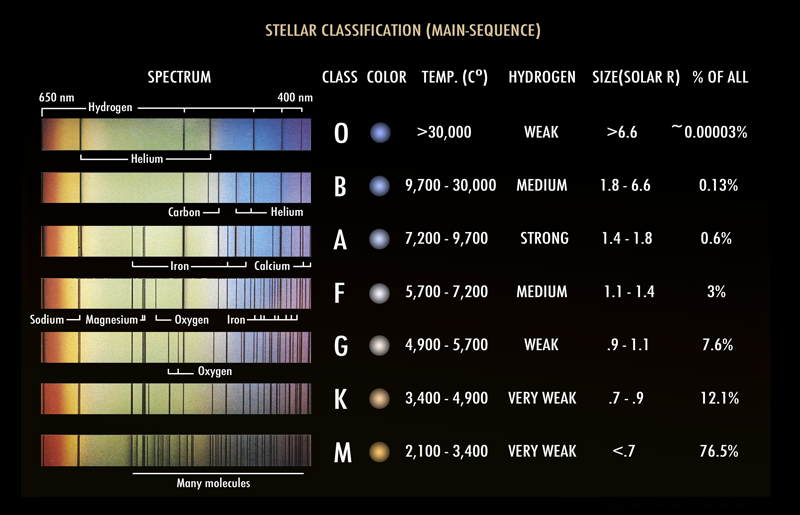
\includegraphics[width=.8\textwidth]{Stellar_Classification_Chart.png}
    \caption{\centering Chart for classifying of the main star types as per the Harvard classification \protect\cite{wikistar}.}
    \label{fig:starclassy}
\end{figure}

Subclasses of numbers ranging from 0-9 allow for finer distinctions in temperature within the OBAFGKM classes. 
For example, the Sun is spectral type \textbf{G2} with a temperature of about 5 700 K (Kelvin) \cite{cosmosstar}.

\subsubsection{MK System of Luminosity}

The Morgan-Keega (MK) Luminosity Class is an addition to the Harvard stellar classification scheme (see §\ref{sec:1.2.1}), given in the form of (primarily) Roman numerals.
This addition to the system was devised in order to be able to distinguish between stars of similar temperatures but differing \textit{luminosities}.

The MK System was originally from I to V, but has since been expanded to differentiate more between I-type stars and further beyond V.
The table containing the luminosity classifications is shown below \cite{mkcosmos}:

\begin{table}[H]
    \centering
    \caption{Table of the MK Luminosity Classes \protect\cite{mkcosmos}.}
    \begin{tabular}{
    |>{\columncolor[HTML]{EFEFEF}}c| c|}
    \hline
    \textbf{Class} & \textbf{Star Type}             \\ \hline
    Ia-O           & extremely luminous supergiants \\
    Ia             & luminous supergiants           \\
    Ib             & less luminous supergiants      \\
    II             & bright giants                  \\
    III            & normal giants                  \\
    IV             & subgiants                      \\
    V              & main sequence dwarf stars      \\
    VI, or sd      & subdwarfs                      \\
    D              & white dwarfs                   \\ \hline            
    \end{tabular}
    \label{tab:1}
\end{table}

\subsubsection{Main Sequence Stars} \label{sec:1.2.2}

Main sequence stars have nuclear reactions at their core through the fusion of hydrogen atoms into helium that allow them to sustain themselves
\cite{schoolmsstar,studymsstar,nasamsstar}.
The radiation pressure from the nuclear reactions and the gravitational pressure work against each other in such a way that the star
remains stable \cite{studymsstar} in a process known as \textbf{hydrostatic equilibrium} \cite{schoolmsstar}.

Figure \ref{fig:msgraphspec} shows the graph of the absorption line spectrum for specific main sequence stars ranging from A to M, excluding classes B and O.

\begin{figure}[H]
    \centering
    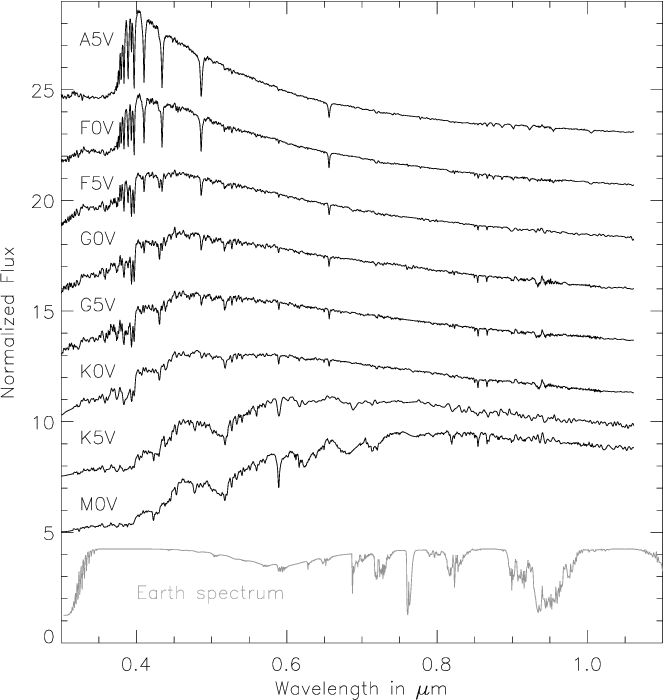
\includegraphics[width=12.5cm]{msspectra.png}
    \caption{\centering Stellar spectra of the main sequence (V) stars (A5 to M0) \protect\cite{msspectrarticle}.}
    \label{fig:msgraphspec}
\end{figure}

\section{Methodology} \label{sec:2}

This experiment made use of the \textit{Contemporary Laboratory Experience in Astronomy}, CLEA, software and the \textit{Classification of Stellar Spectra} program included in the package.
CLEA is an online software developed to simulate and illustrate modern astronomical techniques in a 'real' night sky. This experiment is divided into two separate yet related exercises.
\cite{cleaspectra}.

For the first part of the experiment, graphs of different \textit{absorption spectra} for 25 unknown stars from a list were compared and contrasted against the absorption spectra of main sequence stars of 13 different
spectral types sourced from an Atlas of Standard Spectra. By comparing the known to the unknown, the spectral type for the unknown stars could be approximated and noted. By identifying the approximate
spectral type, astronomers could then estimate the temperature of the star.

The program offered the simulated use of a spectrometer attached to a 0.4m (16") research telescope for the second part of the experiment in which ideally 3 stars are found and studied.
The aim is to find at least both a bright and dim star and utilise the spectrometer attached to the telescope to produce an absorption spectrum for that star. From there, the same as was done for the 
first part of the experiment can be done and the spectral type of the star can be estimated by comparing and contrasting to the Atlas of Standard Spectra provided within the software \cite{UCDspectra}.

Windows for both programs of the experiment are illustrated in figure \ref{fig:program}.

\begin{figure}[H]
    \centering
    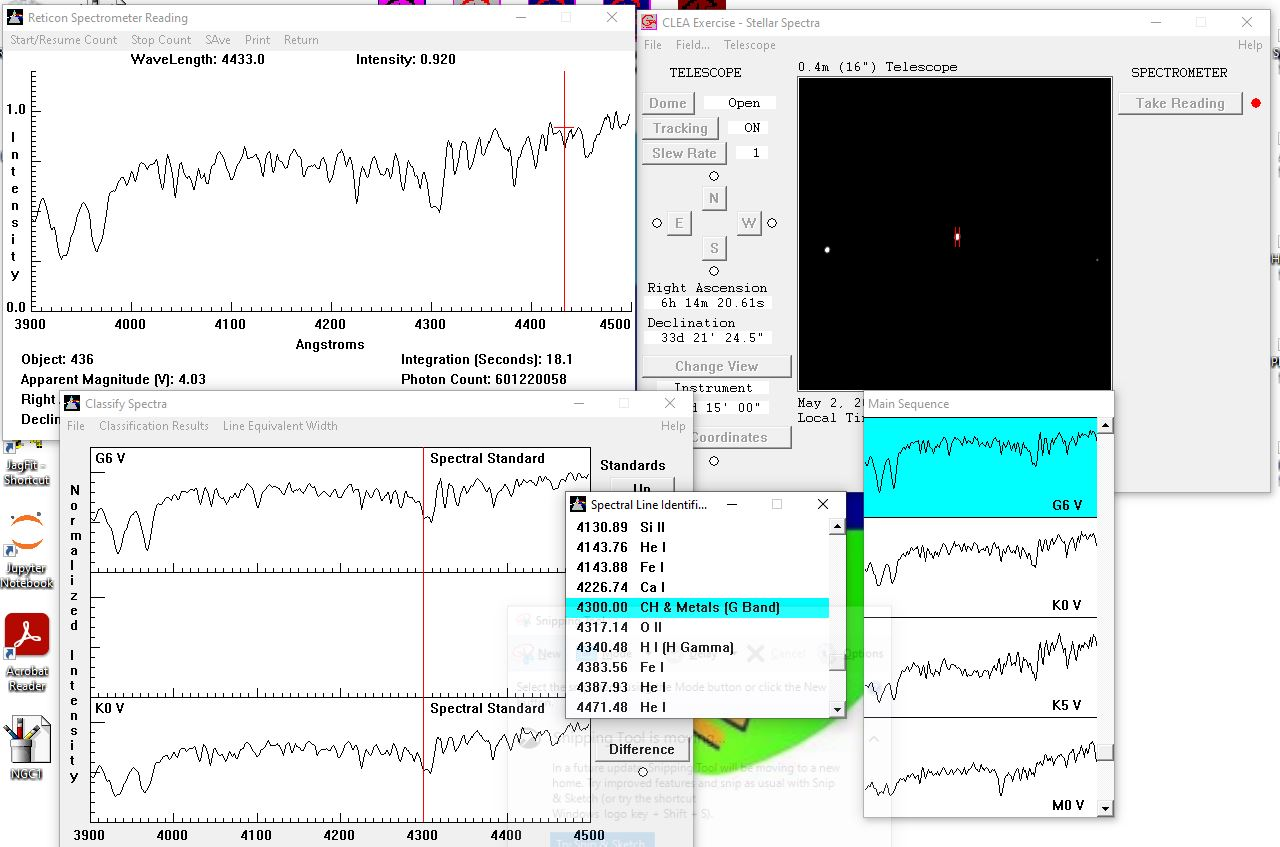
\includegraphics[width=\textwidth]{SPECTRAPIC.JPG}
    \caption{\centering Screenshot of the Stellar Spectra CLEA program.}
    \label{fig:program}
\end{figure}

The spectral type identification program allowed also for the use of different visualisation and data analysis methods (not pictured):

\begin{itemize}
    \item \textbf{Grayscale Photo:} this setting showed a photographed representation of the spectrum in black and white.
    \item \textbf{Graphical Trace:} default setting, graphical representation of the spectra as pictured in figure \ref{fig:program}.
    \item \textbf{Comb. (Photo \& Trace):} combination of both the above settings; centre panel shows the photographic representation of the unknown star whilst the bottom panel shows the graphical representation.
\end{itemize}

These settings are useful to help differentiate between the strongest dips/lines of that spectra when it is not very clear on another representation.

\section{Results and Calculations} \label{sec:3}

\subsection{Spectral Classification (CLEA List)}

The estimated spectral types for the list of the 25 stars provided by CLEA has been formatted into a compact table below, table \ref{tab:2}, with reasons for why that spectral type was chosen for that star:

\begin{table}[H]
    \caption{\centering Table of the estimated spectral class for the CLEA star list, with reasons listed.}
    \label{tab:2}
    \resizebox{\textwidth}{!}{%
        \begin{tabular}{|l|
        >{\columncolor[HTML]{EFEFEF}}c |l|}
        \hline
        \multicolumn{1}{|c|}{\textbf{STAR}} &
        \textbf{SP TYPE} &
        \multicolumn{1}{c|}{\textbf{REASONS}} \\ \hline
        \textbf{HD 124320}  & A3 & HI lines v. strong; Ca II line betw. A1 and A5                  \\ \hline
        \textbf{HD 37767}   & B3 & Strong Ca II lines, He II and HI strong; betw. B0 and B6        \\ \hline
        \textbf{HD 35619}   & O7 & Strong cont. spectrum, weak dips; betw. O5 and B0               \\ \hline
        \textbf{HD 23733}   & F3 & Ca II lines v. strong; betw. F0 and F5                          \\ \hline
        \textbf{O1015}      & B8 & HI lines similar to B6, slightly stronger dips; betw. B6 and A1 \\ \hline
        \textbf{HD 24189}   & G3 & Strong Ca II lines, strong He II line; betw. G0 and G6          \\ \hline
        \textbf{HD 107399}  & F7 & He I line similar to G0; betw. F5 and G0                        \\ \hline
        \textbf{HD 240344}  & B4 & Strong HI line; betw. B0 and B6                                 \\ \hline
        \textbf{HD 17647}   & G5 & Weak HI line, strong Ca II (K) line; betw. G0 and G6            \\ \hline
        \textbf{BD +63 137} & M1 & Strong dip at 4227 Å; betw. M0 and M5                           \\ \hline
        \textbf{HD 66171}   & G5 & Strong Ca II lines, weaker HI (H-gamma); betw. G0 and G6        \\ \hline
        \textbf{HZ 948}     & F7 & Strong HI line, minimal difference slope; betw. F5 and G0       \\ \hline
        \textbf{HD 35215}   & B3 & Strong HI (H-epsilon), minor difference slope; betw. B0 and B6  \\ \hline
        \textbf{Feige 40}   & B4 & Strong HI (H-delta); betw. B0 and B6                            \\ \hline
        \textbf{Feige 41}   & A0 & Strong HI (H-espilon, H-gamma, H-delta) lines; betw. B6 and A1  \\ \hline
        \textbf{HD 6111}    & F8 & Strong Ca II line, strong HI (H-delta) line; betw. F5 and G0    \\ \hline
        \textbf{HD 23863}   & A5 & Smoother cont. spectrum, otherwise identical to A5              \\ \hline
        \textbf{HD 221741}  & A3 & Strong Ca II lines, smoother cont. spectrum; betw. A1 and A5    \\ \hline
        \textbf{HD 242936}  & O5 & Nearly identical to O5                                          \\ \hline
        \textbf{HD 5351}    & K4 & Strong Fe I lines and surrounding dips; betw. K0 and K5         \\ \hline
        \textbf{SAO 81292} &
        M3 &
        \begin{tabular}[c]{@{}l@{}}\textbf{(EMISSION)} v. strong Ca II lines, strong HI (H-gamma); \\ betw. M5 and M0\end{tabular} \\ \hline
        \textbf{HD 27685}   & G6 & Nearly identical to G6                                          \\ \hline
        \textbf{HD 21619}   & A6 & Smoother spectrum; nearly A5                                    \\ \hline
        \textbf{HD 23511}   & F6 & Difference slope slightly below axis; nearly F5                 \\ \hline
        \textbf{HD 158659}  & B0 & V. slightly smoother cont. spectrum; nearly identical to B0     \\ \hline
        \end{tabular}%
    }
\end{table}

The 'HD' prefixed stars are sourced from the \textit{Henry-Draper} catalogue, 'BD' prefixed stars are sourced from the \textit{Bonner Durchmusterung} catalogue, 'HZ' prefixed stars are sourced
from the \textit{Humason-Zwicky} catalogue, 'Feige' prefixed stars are sourced from the \textit{Feige} catalogue, and 'SAO' prefixed stars are sourced from the
\textit{Smithsonian Astrophysical Observatory} catalogue. It is unclear where the 'O' prefixed stars are sourced from.

\subsubsection{SIMBAD Analysis}

The SIMBAD Astronomical Database is made of use to cross-check the stars provided and selected \cite{SIMBAD}. As of the 2nd of March 2025, SIMBAD currently has
20 202 386 objects registered on the database.

\begin{table}[H]
    \caption{Table of the actual spectral types of the CLEA star list as per SIMBAD.}
    \label{tab:4}
    \resizebox{\textwidth}{!}{%
        \begin{tabular}{|l|
        >{\columncolor[HTML]{EFEFEF}}c ||l|
        >{\columncolor[HTML]{EFEFEF}}c ||l|
        >{\columncolor[HTML]{EFEFEF}}c ||l|
        >{\columncolor[HTML]{EFEFEF}}c ||l|
        >{\columncolor[HTML]{EFEFEF}}c |}
        \hline
        \multicolumn{1}{|c|}{\textbf{STAR}} &
        \textbf{\begin{tabular}[c]{@{}c@{}}SP TYPE\\ (SIMBAD)\end{tabular}} &
        \multicolumn{1}{c|}{\textbf{STAR}} &
        \textbf{\begin{tabular}[c]{@{}c@{}}SP TYPE\\ (SIMBAD)\end{tabular}} &
        \multicolumn{1}{c|}{\textbf{STAR}} &
        \textbf{\begin{tabular}[c]{@{}c@{}}SP TYPE\\ (SIMBAD)\end{tabular}} &
        \multicolumn{1}{c|}{\textbf{STAR}} &
        \textbf{\begin{tabular}[c]{@{}c@{}}SP TYPE\\ (SIMBAD)\end{tabular}} &
        \multicolumn{1}{c|}{\textbf{STAR}} &
        \textbf{\begin{tabular}[c]{@{}c@{}}SP TYPE\\ (SIMBAD)\end{tabular}} \\ \hline
        \textbf{HD 124320} &
        A5V &
        \textbf{HD 24189} &
        F6V &
        \textbf{HD 66171} &
        G2V &
        \textbf{HD 6111} &
        G5 E &
        \textbf{SAO 81292} &
        \cellcolor[HTML]{A4DA95}dM3 C \\ \hline
        \textbf{HD 37767} &
        \cellcolor[HTML]{A4DA95}B3V &
        \textbf{HD 107399} &
        G0 E &
        \textbf{HZ 948} &
        N/A &
        \textbf{HD 23863} &
        A7Vn C &
        \textbf{HD 27685} &
        G2 E \\ \hline
        \textbf{HD 35619} &
        \cellcolor[HTML]{A4DA95}O7.5V &
        \textbf{HD 240344} &
        B7 E &
        \textbf{HD 35215} &
        B1V &
        \textbf{HD 221741} &
        A2 E &
        \textbf{HD 21619} &
        \cellcolor[HTML]{A4DA95}A6V C \\ \hline
        \textbf{HD 23733} &
        A9V &
        \textbf{HD 17647} &
        \cellcolor[HTML]{A4DA95}G5 D &
        \textbf{Feige 40} &
        \cellcolor[HTML]{A4DA95}B4V &
        \textbf{HD 242936} &
        A2V &
        \textbf{HD 23511} &
        F5V C \\ \hline
        \textbf{O1015} &
        N/A &
        \textbf{BD +63 137} &
        K7V &
        \textbf{Feige 41} &
        A1V &
        \textbf{HD 5351} &
        \cellcolor[HTML]{A4DA95}K4V C &
        \textbf{HD 158659} &
        B5(Ib/II) D \\ \hline
        \end{tabular}%
    }
\end{table}

Out of the 23 stars available on the SIMBAD database from the 25 of the CLEA list, \textbf{30.4\%} matched what was estimated.

\subsubsection{Jacoby-Hunter-Christian Atlas Analysis}

The Jacoby-Hunter-Christian (JHC) Atlas is made of use to cross-check the stars provided \cite{JHCATLAS}. The JHC Atlas was originally published in 1984 and contains 161 spectra
of stars of spectral classes O to M for luminosity classes V, III, and I.

\begin{table}[H]
    \caption{Table of the actual spectral types of the CLEA star list as per the JHC Atlas.}
    \label{tab:5}
    \resizebox{\textwidth}{!}{%
        \begin{tabular}{|l|
        >{\columncolor[HTML]{EFEFEF}}c ||l|
        >{\columncolor[HTML]{EFEFEF}}c ||l|
        >{\columncolor[HTML]{EFEFEF}}c ||l|
        >{\columncolor[HTML]{EFEFEF}}c ||l|
        >{\columncolor[HTML]{EFEFEF}}c |}
        \hline
        \multicolumn{1}{|c|}{\textbf{STAR}} &
        \textbf{\begin{tabular}[c]{@{}c@{}}SP TYPE\\ (JHC)\end{tabular}} &
        \multicolumn{1}{c|}{\textbf{STAR}} &
        \textbf{\begin{tabular}[c]{@{}c@{}}SP TYPE\\ (JHC)\end{tabular}} &
        \multicolumn{1}{c|}{\textbf{STAR}} &
        \textbf{\begin{tabular}[c]{@{}c@{}}SP TYPE\\ (JHC)\end{tabular}} &
        \multicolumn{1}{c|}{\textbf{STAR}} &
        \textbf{\begin{tabular}[c]{@{}c@{}}SP TYPE\\ (JHC)\end{tabular}} &
        \multicolumn{1}{c|}{\textbf{STAR}} &
        \textbf{\begin{tabular}[c]{@{}c@{}}SP TYPE\\ (JHC)\end{tabular}} \\ \hline
        \textbf{HD 124320} &
        A2V &
        \textbf{HD 24189} &
        F6V &
        \textbf{HD 66171} &
        G2V &
        \textbf{HD 6111} &
        \cellcolor[HTML]{A4DA95}F8V &
        \textbf{SAO 81292} &
        M4.5 Ve \\ \hline
        \textbf{HD 37767} &
        \cellcolor[HTML]{A4DA95}B3V &
        \textbf{HD 107399} &
        F9V &
        \textbf{HZ 948} &
        F3V &
        \textbf{HD 23863} &
        A7V &
        \textbf{HD 27685} &
        G7V \\ \hline
        \textbf{HD 35619} &
        \cellcolor[HTML]{A4DA95}O7V &
        \textbf{HD 240344} &
        \cellcolor[HTML]{A4DA95}B4V &
        \textbf{HD 35215} &
        B1.5V &
        \textbf{HD 221741} &
        \cellcolor[HTML]{A4DA95}A3V &
        \textbf{HD 21619} &
        \cellcolor[HTML]{A4DA95}A6V \\ \hline
        \textbf{HD 23733} &
        A9V &
        \textbf{HD 17647} &
        G1V &
        \textbf{Feige 40} &
        \cellcolor[HTML]{A4DA95}B4V &
        \textbf{HD 242936} &
        N/A &
        \textbf{HD 23511} &
        F4V \\ \hline
        \textbf{O1015} &
        \cellcolor[HTML]{A4DA95}B8V &
        \textbf{BD +63 137} &
        \cellcolor[HTML]{A4DA95}M1V &
        \textbf{Feige 41} &
        A1V &
        \textbf{HD 5351} &
        \cellcolor[HTML]{A4DA95}K4V &
        \textbf{HD 158659} &
        \cellcolor[HTML]{A4DA95}B0V \\ \hline
        \end{tabular}%
        }
\end{table}

Out of the 24 stars available on the JHC Atlas from the 25 of the CLEA list, \textbf{45.8\%} matched what was estimated.

\subsubsection{A Comment on SAO 81292}

During the experiment star SAO 81292 was identified to have emission lines (see figure \ref{fig:swordartonline}).

\begin{figure}[H]
    \centering
    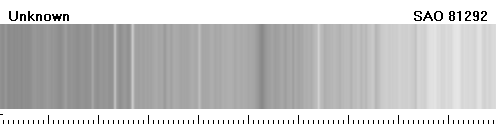
\includegraphics[width=7.5cm]{SAO81292spec.png}
    \caption{\centering Image of the grayscale spectrum for star SAO 81292.}
    \label{fig:swordartonline}
\end{figure}

This could indicate a particularly active late-stage star or a flare star. Through analysis of the lightcurve graph from data gathered by TESS, we can indeed infer that this star is a flare star (see figure \ref{fig:saolight}).

\begin{figure}[H]
    \centering
    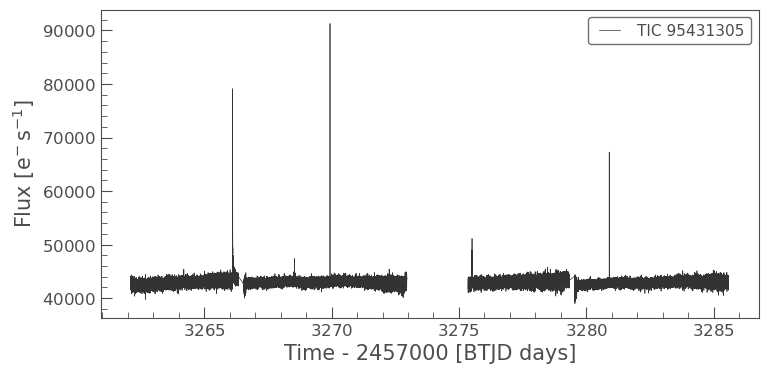
\includegraphics[width=10cm]{SAO lightplot.png}
    \caption{\centering Lightcurve graph plot of the SAO 81292 star, TESS-SPOC data (2023) \protect\cite{TESSSAO}.}
    \label{fig:saolight}
\end{figure}

The flux of light (y-axis) has been gathered over a period of 20 seconds (x-axis), and in that period 4 spikes in the flux can be seen, indicating
flares. Known flare stars have spectral types of late-K through late-M, which is consistent with the information found on both the SIMBAD database and the JHC Atlas.
Additionally, flare stars often have detectable Ca II and H lines, which is also consistent with what was observed from the experiment \cite{aavso}.
As such, SAO 81292 is most likely a flare star and hence the emission lines visible on the spectra in figure \ref{fig:swordartonline}.

\subsection{Spectral Classification (Telescope)}

Three stars, one dim and two bright, were then located on the vast simulated expanse of the sky and the spectrographs for each star was found. Stars were chosen to be relatively far away from
on another and the findings were formatted into a compact table, table \ref{tab:3}, below with the same structure for spectral type and reasoning as before:

\begin{table}[H]
    \caption{\centering Table of the estimated spectral types for self-selected 1 dim and 2 bright stars.}
    \label{tab:3}
    \resizebox{\textwidth}{!}{%
        \begin{tabular}{|
        >{\columncolor[HTML]{EFEFEF}}c |c|c|c|c|c|
        >{\columncolor[HTML]{EFEFEF}}c |l|}
        \hline
        \textbf{\begin{tabular}[c]{@{}c@{}}Star\\ \#\end{tabular}} &
        \textbf{\begin{tabular}[c]{@{}c@{}}Star\\ Name\end{tabular}} &
        \textbf{\begin{tabular}[c]{@{}c@{}}RA\\ (h  m  s)\end{tabular}} &
        \textbf{\begin{tabular}[c]{@{}c@{}}DE\\ (d  m  s)\end{tabular}} &
        \textbf{\begin{tabular}[c]{@{}c@{}}App. \\ Mag. (m)\end{tabular}} &
        \textbf{\begin{tabular}[c]{@{}c@{}}S/N\\ Ratio\end{tabular}} &
        \textbf{\begin{tabular}[c]{@{}c@{}}SP\\ Type\end{tabular}} &
        \textbf{Reasons} \\ \hline
        \textbf{1} &
        436 &
        6  14  20 &
        33  21  24 &
        4.03 &
        1001 &
        G7 &
        \begin{tabular}[c]{@{}l@{}}Strong Ca II lines, strong G-band; \\ betw. G6 and K0\end{tabular} \\ \hline
        \textbf{2} &
        57 &
        6  22  28 &
        30  52  21 &
        14.65 &
        45 &
        A6 &
        \begin{tabular}[c]{@{}l@{}}Sharper dips, noisy (S/N ratio); \\ betw. A5 and F0\end{tabular} \\ \hline
        \textbf{3} &
        49 &
        6  07  19 &
        30  12  32 &
        5.98 &
        879 &
        B5 &
        \begin{tabular}[c]{@{}l@{}}Strong H I (H-epsilon, H-delta, H-gamma) \\ lines, stronger Fe I line; \\ betw. B0 and B6\end{tabular} \\ \hline
        \end{tabular}%
    }
\end{table}

It was important to get the S/N (signal to noise) ratio of each specturm to be as low as possible (higher number) so the spectra would not be as noisy. If the spectrum
is noisy, it is much harder to identify the most prominent absorption lines. This can be helped by choosing to use a larger telescope (CLEA offers both 1.0m and 4.0m telescopes to be used) as this
way the telescope can collect more light quicker, reducing the noise present in the spectrograph. 

\subsubsection{SIMBAD Analysis}

Much like before, the SIMBAD database can be made of use to cross-check the stars found on the digitally simulated nightsky provided by CLEA by inputing
the RA and DE coordinates found.

\begin{table}[H]
    \centering
    \caption{Stars found through telescope cross-matched on SIMBAD to a radius of 5 arc min.}
    \label{tab:6}
    \resizebox{.75\textwidth}{!}{%
    \begin{tabular}{|
    >{\columncolor[HTML]{EFEFEF}}c |c|c|c|c|
    >{\columncolor[HTML]{EFEFEF}}c |}
    \hline
    \textbf{\begin{tabular}[c]{@{}c@{}}Star\\ \#\end{tabular}} &
      \textbf{\begin{tabular}[c]{@{}c@{}}Star\\ Name\end{tabular}} &
      \textbf{\begin{tabular}[c]{@{}c@{}}RA\\ (h m s)\end{tabular}} &
      \textbf{\begin{tabular}[c]{@{}c@{}}DE\\ (d m s)\end{tabular}} &
      \textbf{\begin{tabular}[c]{@{}c@{}}Mag. \\ (unspecified)\end{tabular}} &
      \textbf{\begin{tabular}[c]{@{}c@{}}SP Type\\ (SIMBAD)\end{tabular}} \\ \hline
    \textbf{1} & HD 253515   & 6 14 \textbf{26}          & +33 21 \textbf{01}          & 11.3  & kA1hA2mA3 \\ \hline
    \textbf{2} & HD 44300    & 6 22 28          & +30 \textbf{56 43} & 8.82  & F0        \\ \hline
    \textbf{3} & EM* MWC 790 & 6 07 \textbf{24} & +30 \textbf{11 44} & 12.77 & Be        \\ \hline
    \end{tabular}%
    }
\end{table}

The change in coordinates from those gathered has been highlighted in bold, and only the results where the spectral type was provided have been taken (as it is the aim of the experiment).

According to SIMBAD, star 1 (HD 253515) is of spectral type kA1hA2mA3. This is an Am (metallic-lined) A star with Ca II K-line bands corresponding to that of an A1 spectral type,
Hydrogen (H) lines corresponding to that of an A2 spectral type, and metallic lines (such as Iron (Fe)) corresponding to that of an A3 spectral type. Am stars are chemically peliculiar, hence 
the deviation from standard spectral type classification.

Also accoding to SIMBAD \cite{SIMBADguide}, the lowercase 'e' that follows star 3's (EM* MWC 790) spectral type B indicates emission lines in the spectrum.

\subsubsection{(ADDITIONAL) Spectral Classification (SIMBAD Coordinates)}

With reference to these new SIMBAD coordinates instead, the telescope was accessed again (not in the laboratory) and the experiment was done again to cross-check. As this new rendition of the experiment was not done in
the laboratory, the newest version of the CLEA VIREO (VIRtual Educational Observatory) software was able to be accessed. This version allows for a much wider expanse of the simulated nightsky to be observed, the following results were obtained:

\begin{table}[H]
    \caption{\centering Estimated spectral types of stars as per the SIMBAD approximate coordinates \newline (non-laboratory rendition).}
    \label{tab:7}
    \resizebox{\textwidth}{!}{%
    \begin{tabular}{|
    >{\columncolor[HTML]{EFEFEF}}c |c|c|c|c|c|
    >{\columncolor[HTML]{EFEFEF}}c |l|}
    \hline
    \textbf{\begin{tabular}[c]{@{}c@{}}Star\\ \#\end{tabular}} &
      \textbf{\begin{tabular}[c]{@{}c@{}}Object\\ Name\end{tabular}} &
      \textbf{\begin{tabular}[c]{@{}c@{}}RA\\ (h m s)\end{tabular}} &
      \textbf{\begin{tabular}[c]{@{}c@{}}DE\\ (d m s)\end{tabular}} &
      \textbf{\begin{tabular}[c]{@{}c@{}}App. \\ Mag. (m)\end{tabular}} &
      \textbf{\begin{tabular}[c]{@{}c@{}}S/N\\ Ratio\end{tabular}} &
      \textbf{\begin{tabular}[c]{@{}c@{}}SP\\ Type\end{tabular}} &
      \textbf{Reasons} \\ \hline
    \textbf{1} &
      N3000-01024 &
      6 14 26.1 &
      +33 21 01 &
      11.63 &
      521 &
      B8 &
      \begin{tabular}[c]{@{}l@{}}Strong HI (H-gamma) line, strong He II line; \\ betw. B6 and A1\end{tabular} \\ \hline
    \textbf{2} &
      N3000-00640 &
      6 22 28.4 &
      +30 56 43 &
      8.35 &
      1000 &
      F0 &
      Identical to F0 \\ \hline
    \textbf{3} &
      N3000-01059 &
      6 07 23.7 &
      +30 11 42 &
      11.67 &
      620 &
      A3 &
      \begin{tabular}[c]{@{}l@{}}Slightly weaker Ca II (K) line; \\ betw. A1 and A5\end{tabular} \\ \hline
    \end{tabular}%
    }
\end{table}

This addition to the experiment was not necessary, but merely a means to compare the data gathered from the SIMBAD database to what would have been obtained
from the laboratory experiment. Identical approaches were taken, different softwares and settings. 

\newpage

\section{Conclusion} \label{sec:4}

Through the use of the CLEA software, this experiment was successful in practicing classifying spectral types of stars based on this spectra. When compared to two different
databases, it was found that \textbf{30.4\%} of the estimated spectral types matched with the SIMBAD database, while \textbf{45.8\%} of the estimated spectral
types matched with the JHC Atlas. The fact that these results do not match could be due to discrepancies in data-gathering methods and complexities of the stars, or classification threshold differences as
SIMBAD has a lot more variable descriptors for spectral types.

For the telescope-based section of the experiment, the same approach as before was taken. The factor of the signal-to-noise ratio meant that there was likely some
error in estimating the spectral type for stars as some spectral types are more reliant on the 'smoothness' of the spectrum. Higher ratios also meant more noise, making it difficult to tell
what were the most prominent lines of the absorption spectrum. This issue could be fixed by making use of the larger telescopes available within the software.

\newpage

%%%%%%%%%%%%%%%%%%%%%%%%%%%%%%%%%%%

\bibliographystyle{IEEEtran}
{\footnotesize\bibliography{References}} \label{sec:ref}

\vspace{1.5cm}

\listoffigures

\listoftables

\vspace{2.5cm}

\section*{Appendix} \label{sec:A}
\addcontentsline{toc}{section}{Appendix}

\subsection*{Code}
\addcontentsline{toc}{subsection}{Code}

%

\begin{minipage}{\linewidth}
\captionsetup{hypcap=false}

\begin{mintedbox}
\begin{minted}[fontsize=\small, breaklines, baselinestretch=1.2, xleftmargin=0.5cm]{python}
import matplotlib.pyplot as plt
import lightkurve as lk
%matplotlib inline # thank you to https://www.youtube.com/watch?v=fhQjDv_vuQU

data = lk.search_lightcurve("SAO 81292", mission = "TESS")
data

lc = data.download_all()
lc[6].plot() # from data table, [6]: exptime 20s, year 2023, author SPOC

\end{minted}
\end{mintedbox}

\captionof*{figure}{\centering Code for generating the lightcurve graph in figure \ref{fig:saolight}.}
\end{minipage}

\begin{figure}[H]
    \centering
    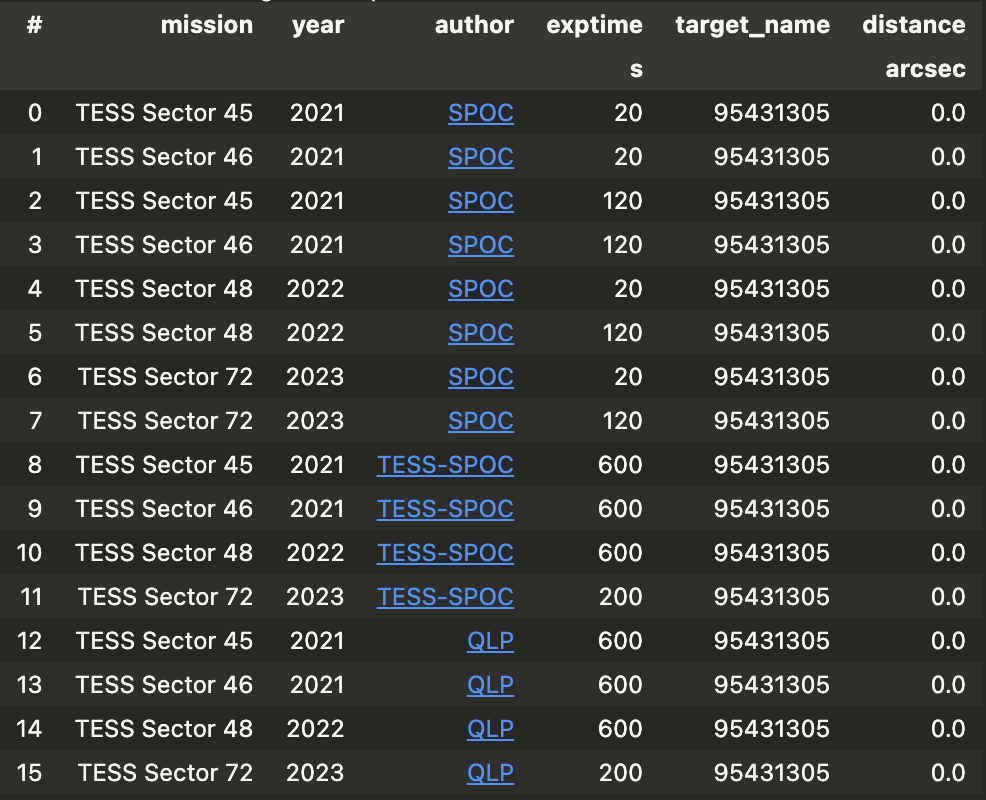
\includegraphics[width=\textwidth]{SAO tess data.png}
    \caption*{\centering Data table sourced with the code from TESS.}
\end{figure}

\newpage

\subsection*{CLEA Atlas of Standard Spectra}
\addcontentsline{toc}{subsection}{CLEA Atlas of Standard Spectra}

\begin{figure}[H]
    \centering
    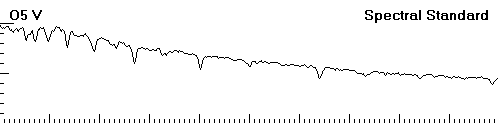
\includegraphics[width=.47\textwidth]{O5V.png}
    \caption*{\centering Atlas of Standard Spectra: \textbf{O5}}
\end{figure}
\vspace{-1.5ex}
\begin{minipage}{.47\textwidth}
    \captionsetup{hypcap=false}
    \centering
    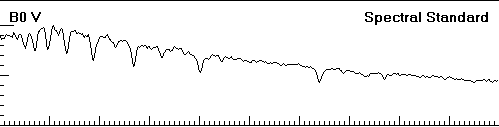
\includegraphics[width=\linewidth]{B0V.png}
    \captionof*{figure}{\centering Atlas of Standard Spectra: \textbf{B0}}

    \vfill
    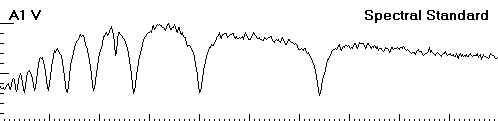
\includegraphics[width=\linewidth]{A1V.png}
    \captionof*{figure}{\centering Atlas of Standard Spectra: \textbf{A1}}

    \vfill
    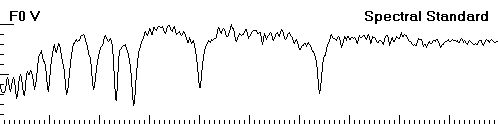
\includegraphics[width=\linewidth]{F0V.png}
    \captionof*{figure}{\centering Atlas of Standard Spectra: \textbf{F0}}

    \vfill
    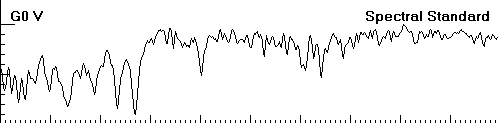
\includegraphics[width=\linewidth]{G0V.png}
    \captionof*{figure}{\centering Atlas of Standard Spectra: \textbf{G0}}

    \vfill
    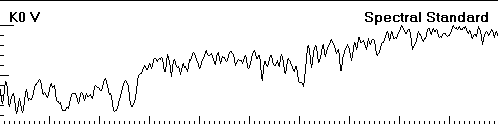
\includegraphics[width=\linewidth]{K0V.png}
    \captionof*{figure}{\centering Atlas of Standard Spectra: \textbf{K0}}

    \vfill
    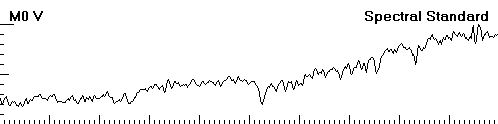
\includegraphics[width=\linewidth]{M0V.png}
    \captionof*{figure}{\centering Atlas of Standard Spectra: \textbf{M0}}
\end{minipage}
\hfill
\begin{minipage}{.47\textwidth}
    \captionsetup{hypcap=false}
    \centering
    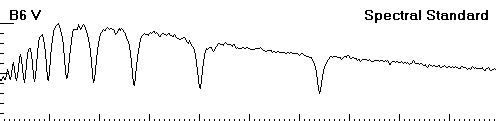
\includegraphics[width=\linewidth]{B6V.png}
    \captionof*{figure}{\centering Atlas of Standard Spectra: \textbf{B6}}

    \vfill
    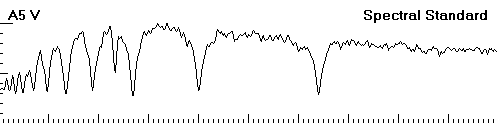
\includegraphics[width=\linewidth]{A5V.png}
    \captionof*{figure}{\centering Atlas of Standard Spectra: \textbf{A5}}

    \vfill
    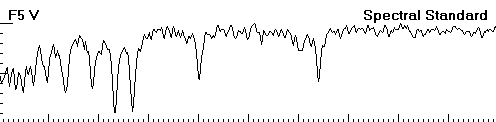
\includegraphics[width=\linewidth]{F5V.png}
    \captionof*{figure}{\centering Atlas of Standard Spectra: \textbf{F5}}

    \vfill
    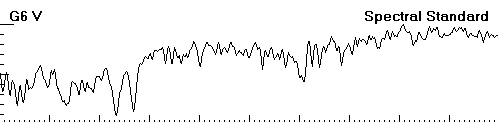
\includegraphics[width=\linewidth]{G6V.png}
    \captionof*{figure}{\centering Atlas of Standard Spectra: \textbf{G6}}

    \vfill
    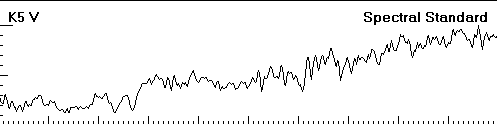
\includegraphics[width=\linewidth]{K5V.png}
    \captionof*{figure}{\centering Atlas of Standard Spectra: \textbf{K5}}

    \vfill
    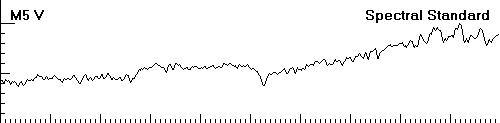
\includegraphics[width=\linewidth]{m5V.png}
    \captionof*{figure}{\centering Atlas of Standard Spectra: \textbf{M5}}
\end{minipage}

\end{document}